% !TeX root = ../main.tex
% reduce display equation skip
\setlength{\abovedisplayskip}{4pt}
\setlength{\belowdisplayskip}{4pt}
\setlength{\textfloatsep}{4pt}

The architecture and training procedures of neural networks have rapidly evolved in recent years. In this section we identify some recent changes that are responsible for the miscalibration phenomenon observed in \autoref{figure.complenet}.
Though we cannot claim causality, we find that increased model capacity and lack of regularization are closely related to model miscalibration.

% which produces well-calibrated probability scores in traditional settings {\color{red} (cite, cite, cite)}. Indeed, many applications have historically been using these $p_k\in[0,1]$ as actual probabilities \citep{girshick2015fast} {\color{red} (cite)}. In fact, an empirical survey by Niculescu-Mizil and Caruana \citet{niculescu2005predicting} ranked neural networks among the most calibrated models.

% However, a decade has gone by, and as we have already introduced in \autoref{introduction}, deep networks nowadays are poorly calibrated. Following the training recipe exactly as provided by the authors, we observe severe \emph{overconfidence} on various models with state-of-the-art accuracy. In this section we will explore the cause of this phenomenon.
%Here we outline what trends may be causing this miscalibration.
%It'll be important to emphasize that we are not trying to explain why these
%trends cause miscalibration, rather that we are just noticing these trends.

\paragraph{Model capacity.}
The model capacity of neural networks has increased at a dramatic pace over the past few years. It is now common to see networks with hundreds, if not thousands of layers \cite{he2015deep,huang2016deep} and hundreds of convolutional filters per layer \cite{zagoruyko2016wide}. Recent work shows that very deep or wide models are able to generalize better than smaller ones, while exhibiting the capacity to easily fit the training set \cite{zhang2016understanding}.

Although increasing depth and width may reduce classification error, we observe that these increases negatively affect model calibration.
\autoref{figure.factors} displays error and ECE as a function of depth and width on a ResNet trained on CIFAR-100. The far left figure varies depth for a network with 64 convolutional filters per layer, while the middle left figure fixes the depth at 14 layers and varies the number of convolutional filters per layer. Though even the smallest models in the graph exhibit some degree of miscalibration, the ECE metric grows substantially with model capacity.
During training, after the model is able to correctly classify (almost) all training samples, NLL can be further minimized by increasing the confidence of predictions.
Increased model capacity will lower training NLL, and thus the model will be more (over)confident on average.
% We observe that these models also output overly confident probabilities on test samples.
% This trend is also prominent among many other datasets and model architectures.
% Results and figures on the other datasets are included in the supplementary material.

\paragraph{Batch Normalization} \cite{ioffe2015batch} improves the optimization of neural networks by minimizing distribution shifts in activations within the neural network's hidden layers. Recent research suggests that these normalization techniques have enabled the development of very deep architectures, such as ResNets \cite{he2015deep} and DenseNets \cite{huang2016densely}. It has been shown that Batch Normalization improves training time, reduces the need for additional regularization, and can in some cases improve the accuracy of networks.

While it is difficult to pinpoint exactly how Batch Normalization affects the final predictions of a model, we do observe that models trained with Batch Normalization tend to be more miscalibrated. In the middle right plot of \autoref{figure.factors}, we see that a 6-layer ConvNet obtains worse calibration when Batch Normalization is applied, even though classification accuracy improves slightly. We find that this result holds regardless of the hyperparameters used on the Batch Normalization model (i.e. low or high learning rate, etc.).
% It is difficult to attribute the cause of this phenomenon to any particular effect of Batch Normalization.

\begin{figure}[t!]
	\centering
	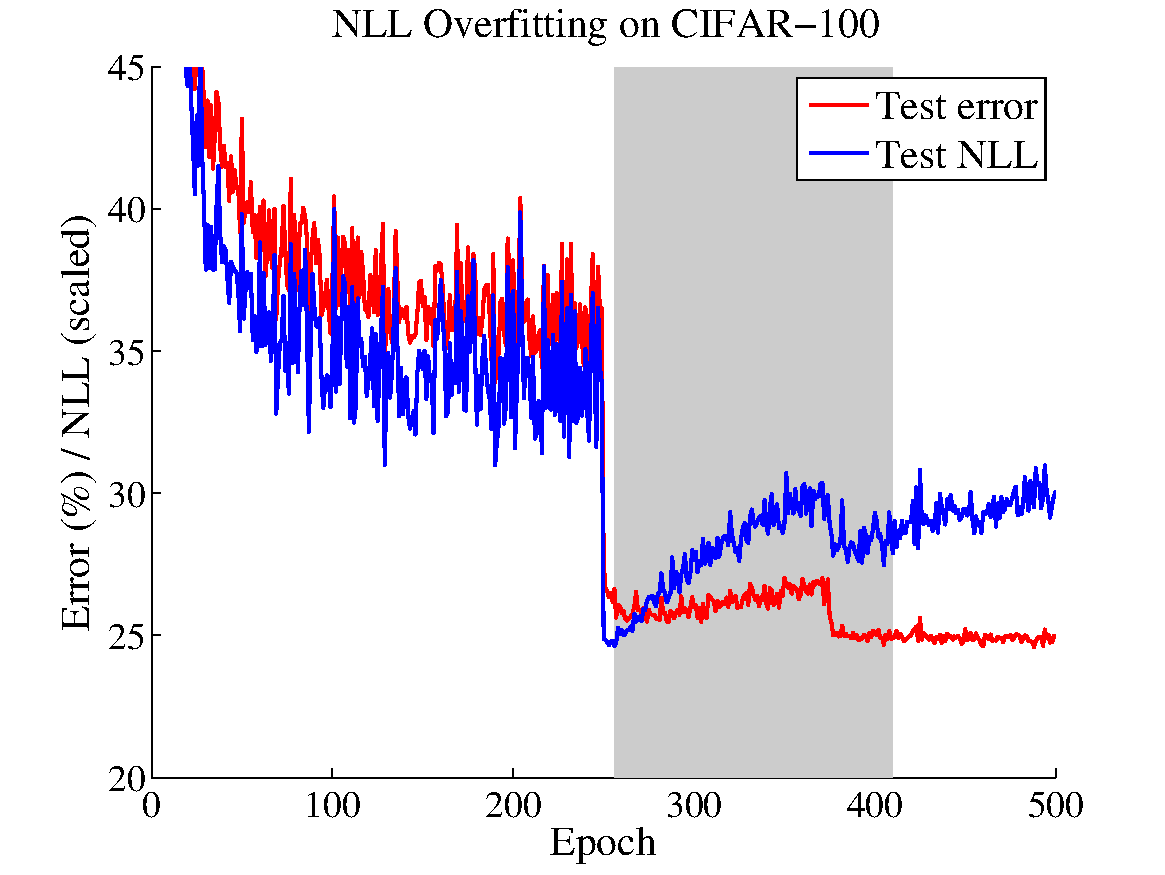
\includegraphics[width=\columnwidth]{fig/cifar100_overfit.pdf}
	\caption{Test error and NLL of a 110-layer ResNet with stochastic depth on CIFAR-100 during training. NLL is scaled by a constant to fit in the figure. Learning rate drops by 10x at epochs 250 and 375. The shaded area marks between epochs at which the best validation \emph{loss} and best validation \emph{error} are produced.}
	\label{figure.cifar100_overfit}
	\vspace{1ex}
\end{figure}

\paragraph{Weight decay,} which used to be the predominant regularization mechanism for neural networks, is decreasingly utilized when training modern neural networks. Learning theory suggests that regularization is necessary to prevent overfitting, especially as model capacity increases \cite{vapnik1998}. However, due to the apparent regularization effects of Batch Normalization, recent research seems to suggest that models with less L2 regularization tend to generalize better \cite{ioffe2015batch}. As a result, it is now common to train models with little weight decay, if any at all. The top performing ImageNet models of 2015 all use an order of magnitude less weight decay than models of previous years \cite{he2015deep, simonyan2014very}.

We find that training with less weight decay has a negative impact on calibration.
The far right plot in \autoref{figure.factors} displays training error and ECE for a 110-layer ResNet with varying amounts of weight decay.
The only other forms of regularization are data augmentation and Batch Normalization.
We observe that calibration and accuracy are not optimized by the same parameter setting.
While the model exhibits both over-regularization and under-regularization with respect to classification error, it does not appear that calibration is negatively impacted by having too much weight decay.
Model calibration continues to improve when more regularization is added, well after the point of achieving optimal accuracy.
The slight uptick at the end of the graph may be an artifact of using a weight decay factor that impedes optimization.

\paragraph{NLL} can be used to indirectly measure model calibration. In practice, we observe \emph{a disconnect between NLL and accuracy}, which may explain the miscalibration in \autoref{figure.factors}.
%
This disconnect occurs because neural networks can \emph{overfit to NLL without overfitting to the 0/1 loss}.
We observe this trend in the training curves of some miscalibrated models.
\autoref{figure.cifar100_overfit} shows test error and NLL (rescaled to match error) on CIFAR-100 as training progresses.
Both error and NLL immediately drop at epoch 250, when the learning rate is dropped; however, NLL overfits during the remainder of training.
Surprisingly, overfitting to NLL is beneficial to classification accuracy. On CIFAR-100, test error drops from $29\%$ to $27\%$ in the region where NLL overfits. This phenomenon renders a concrete explanation of miscalibration: the network learns better classification accuracy at the expense of well-modeled probabilities.

We can connect this finding to recent work examining the generalization of large neural networks. \citet{zhang2016understanding} observe that deep neural networks seemingly violate  the common understanding of learning theory that large models with little regularization will not generalize well. The observed disconnect between NLL and 0/1 loss suggests that these high capacity models are not necessarily immune from overfitting, but rather, overfitting manifests in probabilistic error rather than classification error.
%Though we are not able to explain why this disconnect occurs, it does offer intuition as to why modern neural networks tend to be miscalibrated.
